% This file was created with tikzplotlib v0.10.1.
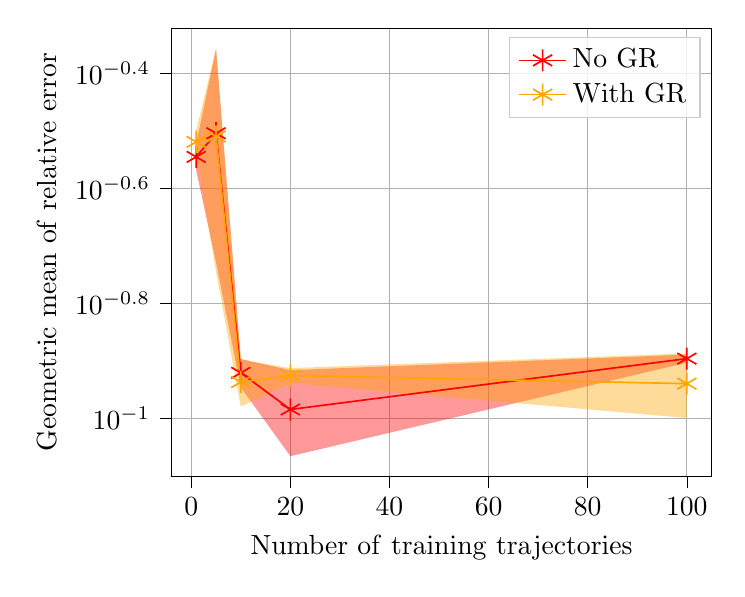
\begin{tikzpicture}

\definecolor{darkgray176}{RGB}{176,176,176}
\definecolor{lightgray204}{RGB}{204,204,204}
\definecolor{orange}{RGB}{255,165,0}

\begin{axis}[
legend cell align={left},
legend style={fill opacity=0.8, draw opacity=1, text opacity=1, draw=lightgray204},
log basis y={10},
tick align=outside,
tick pos=left,
x grid style={darkgray176},
xlabel={\(\displaystyle \mathrm{Number \ of \ training \ trajectories }\)},
xmajorgrids,
xmin=-3.95, xmax=104.95,
xtick style={color=black},
y grid style={darkgray176},
ylabel={\(\displaystyle \mathrm{Geometric \ mean \ of \ relative \ error }\)},
ymajorgrids,
ymin=0.0793577002242894, ymax=0.477073682708961,
ymode=log,
ytick style={color=black}
]
\path [fill=red, fill opacity=0.4, semithick]
(axis cs:1,0.300120892829339)
--(axis cs:1,0.270117436464185)
--(axis cs:5,0.187016546987665)
--(axis cs:10,0.113334387438844)
--(axis cs:20,0.0860989787528075)
--(axis cs:100,0.125133298536034)
--(axis cs:100,0.129239593406028)
--(axis cs:100,0.129239593406028)
--(axis cs:20,0.121457346805786)
--(axis cs:10,0.126990451979335)
--(axis cs:5,0.439720317775325)
--(axis cs:1,0.300120892829339)
--cycle;

\path [fill=orange, fill opacity=0.4, semithick]
(axis cs:1,0.317190999284616)
--(axis cs:1,0.288253249502251)
--(axis cs:5,0.180009995179042)
--(axis cs:10,0.105024693862088)
--(axis cs:20,0.115317977754278)
--(axis cs:100,0.100280781002313)
--(axis cs:100,0.129872046553742)
--(axis cs:100,0.129872046553742)
--(axis cs:20,0.12245994606289)
--(axis cs:10,0.126613268772451)
--(axis cs:5,0.438831211225539)
--(axis cs:1,0.317190999284616)
--cycle;

\addplot [semithick, red, mark=asterisk, mark size=4, mark options={solid}]
table {%
1 0.285119146108627
5 0.313368439674377
10 0.120162419974804
20 0.103778138756752
100 0.127186432480812
};
\addlegendentry{No GR}
\addplot [semithick, orange, mark=asterisk, mark size=4, mark options={solid}]
table {%
1 0.302722126245499
5 0.309420585632324
10 0.115819007158279
20 0.118888966739178
100 0.115076400339603
};
\addlegendentry{With GR}
\end{axis}

\end{tikzpicture}
